\documentclass[final,paperwidth=36in,paperheight=48in,portrait,fontscale=0.3]{baposter}
% NIPS Workshops format

% Encoding.
\usepackage[utf8]{inputenc}
\usepackage[T1]{fontenc}

\usepackage{graphicx} % Required for including images
\usepackage{subfig}
\usepackage{booktabs} % for professional tables
\usepackage{floatrow}
\usepackage{float}

\usepackage{textgreek}
\usepackage{pstricks}
\usepackage{tikz}
\usepackage{pgf}
\usepackage{multirow}
\usepackage{wrapfig}
\usepackage{multicol}
\usepackage{placeins} % For \FloatBarrier
\usetikzlibrary{positioning}
\usepackage{environ}
\makeatletter
\newsavebox{\measure@tikzpicture}
\NewEnviron{scaletikzpicturetowidth}[1]{%
	\def\tikz@width{#1}%
	\def\tikzscale{1}\begin{lrbox}{\measure@tikzpicture}%
		\BODY
	\end{lrbox}%
	\pgfmathparse{#1/\wd\measure@tikzpicture}%
	\edef\tikzscale{\pgfmathresult}%
	\BODY
}
\makeatother

\usepackage{amsmath} % For typesetting math
\usepackage{amssymb} % Adds new symbols to be used in math mode

\usepackage{booktabs} % Top and bottom rules for tables
\usepackage{enumitem} % Used to reduce itemize/enumerate spacing
%\usepackage{palatino} % Use the Palatino font
\renewcommand{\familydefault}{\sfdefault}
\usepackage[font=small,labelfont=bf]{caption} % Required for specifying captions to tables and figures

\usepackage{multicol} % Required for multiple columns
\setlength{\columnsep}{1.5em} % Slightly increase the space between columns
\setlength{\columnseprule}{0mm} % No horizontal rule between columns
\usepackage{multirow}
\usepackage{graphicx}

% For gap between cmidrules.
\usepackage{array}
\newcolumntype{C}{@{\extracolsep{0.1cm}}c@{\extracolsep{0pt}}}%

\setlength{\columnsep}{1cm}
\setlength{\columnseprule}{0.5pt}
\def\columnseprulecolor{\color{Plum}}


\newcommand{\compresslist}{ % Define a command to reduce spacing within itemize/enumerate environments, this is used right after \begin{itemize} or \begin{enumerate}
\setlength{\itemsep}{1pt}
\setlength{\parskip}{0pt}
\setlength{\parsep}{0pt}
}

% Defines the color used for content box headers
\definecolor{lightblue}{cmyk}{0.83,0.24,0,0.16}
%\definecolor{lightblue}{rgb}{0.145,0.6666,1}

%%%%%%%%%%%%%%%%%%%%%%%%%%%%%%%%%%%%%%%%%%%%%%%%%%%%%%%%%%%%%%%%%%%%%%%%%%%%%%
%%% Begin of Document
%%%%%%%%%%%%%%%%%%%%%%%%%%%%%%%%%%%%%%%%%%%%%%%%%%%%%%%%%%%%%%%%%%%%%%%%%%%%%%

% Pojedyncze spacje po kropce.
\frenchspacing

\begin{document}



\hyphenation{resolution occlusions}
%%
\begin{poster}%
  % Poster Options
  {
  % Show grid to help with alignment
  grid=false,
  % Column spacing
  colspacing=1em,
  % Color style
  bgColorOne=white,
  bgColorTwo=white,
  borderColor=lightblue,
  headerColorOne=black,
  headerColorTwo=lightblue,
  headerFontColor=white,
  boxColorOne=white,
  boxColorTwo=lightblue,
  % Format of textbox
  textborder=roundedleft,
%  textborder=faded,
  % Format of text header
  eyecatcher=true,
  headerborder=closed,
  columns=2,
  headerheight=4cm,
%  textfont=\sc, An example of changing the text font
  headershape=roundedright,
  headershade=shadelr,
  headerfont=\Large\bf\textsc, %Sans Serif
  textfont={\setlength{\parindent}{1.5em}\large},
  boxshade=plain,
%  background=shade-tb,
  background=plain,
  linewidth=1pt
  } 
  { % Left Eye Catcher - IBM logo

\includegraphics[width=4cm]{../img/ibm_research.png}
  } 
  % Title
  	{\bf\textsc{On transfer learning using a MAC model variant}\vspace{0.2em}}
  % Authors
  {
	\textbf{Vincent Marois, T.S. Jayram, Vincent Albouy, Tomasz Kornuta, \\Younes Bouhadjar, Ahmet S. Ozcan}\\

	\texttt{\{vmarois,jayram,tkornut,byounes,asozcan\}@us.ibm.com},{\{vincent.albouy\}@ibm.com}\\
  }
  { % Left Eye Catcher

\includegraphics[width=4cm]{../img/arc_logo.png}
  }


% A coloured circle useful as a bullet with an adjustably strong filling
\newcommand{\colouredcircle}{%
\tikz{\useasboundingbox (-0.2em,-0.32em) rectangle(0.2em,0.32em); \draw[draw=black,fill=lightblue,line width=0.03em] (0,0) circle(0.16em);}}
\tikzstyle{block} = [draw,minimum size=2.5em, outer sep=2]

%%%%%%%%%%%%%%%%%%%%%%%%%%%%%%%%%%%%%%%%%%%%%%%%%%%%%%%%%%%%%%%%%%%%%%%%%%%%%%%

\headerbox{Abstract}{name=abstract,column=0,row=0}{
We introduce a variant of the MAC model (Hudson and Manning, ICLR 2018) with a simplified set of equations that achieves comparable accuracy, while training faster. We evaluate both models on CLEVR and CoGenT, and show that, transfer learning with fine-tuning results in a 15 point increase in accuracy, matching the state of the art. Finally, in contrast, we demonstrate that improper fine-tuning can actually reduce a model's accuracy as well.
} %headerbox

\headerbox{The MAC Model}{name=double-pendulum, column=0, below=abstract}{
	\begin{figure}[H]
		\centering
		\subfloat[]{{
				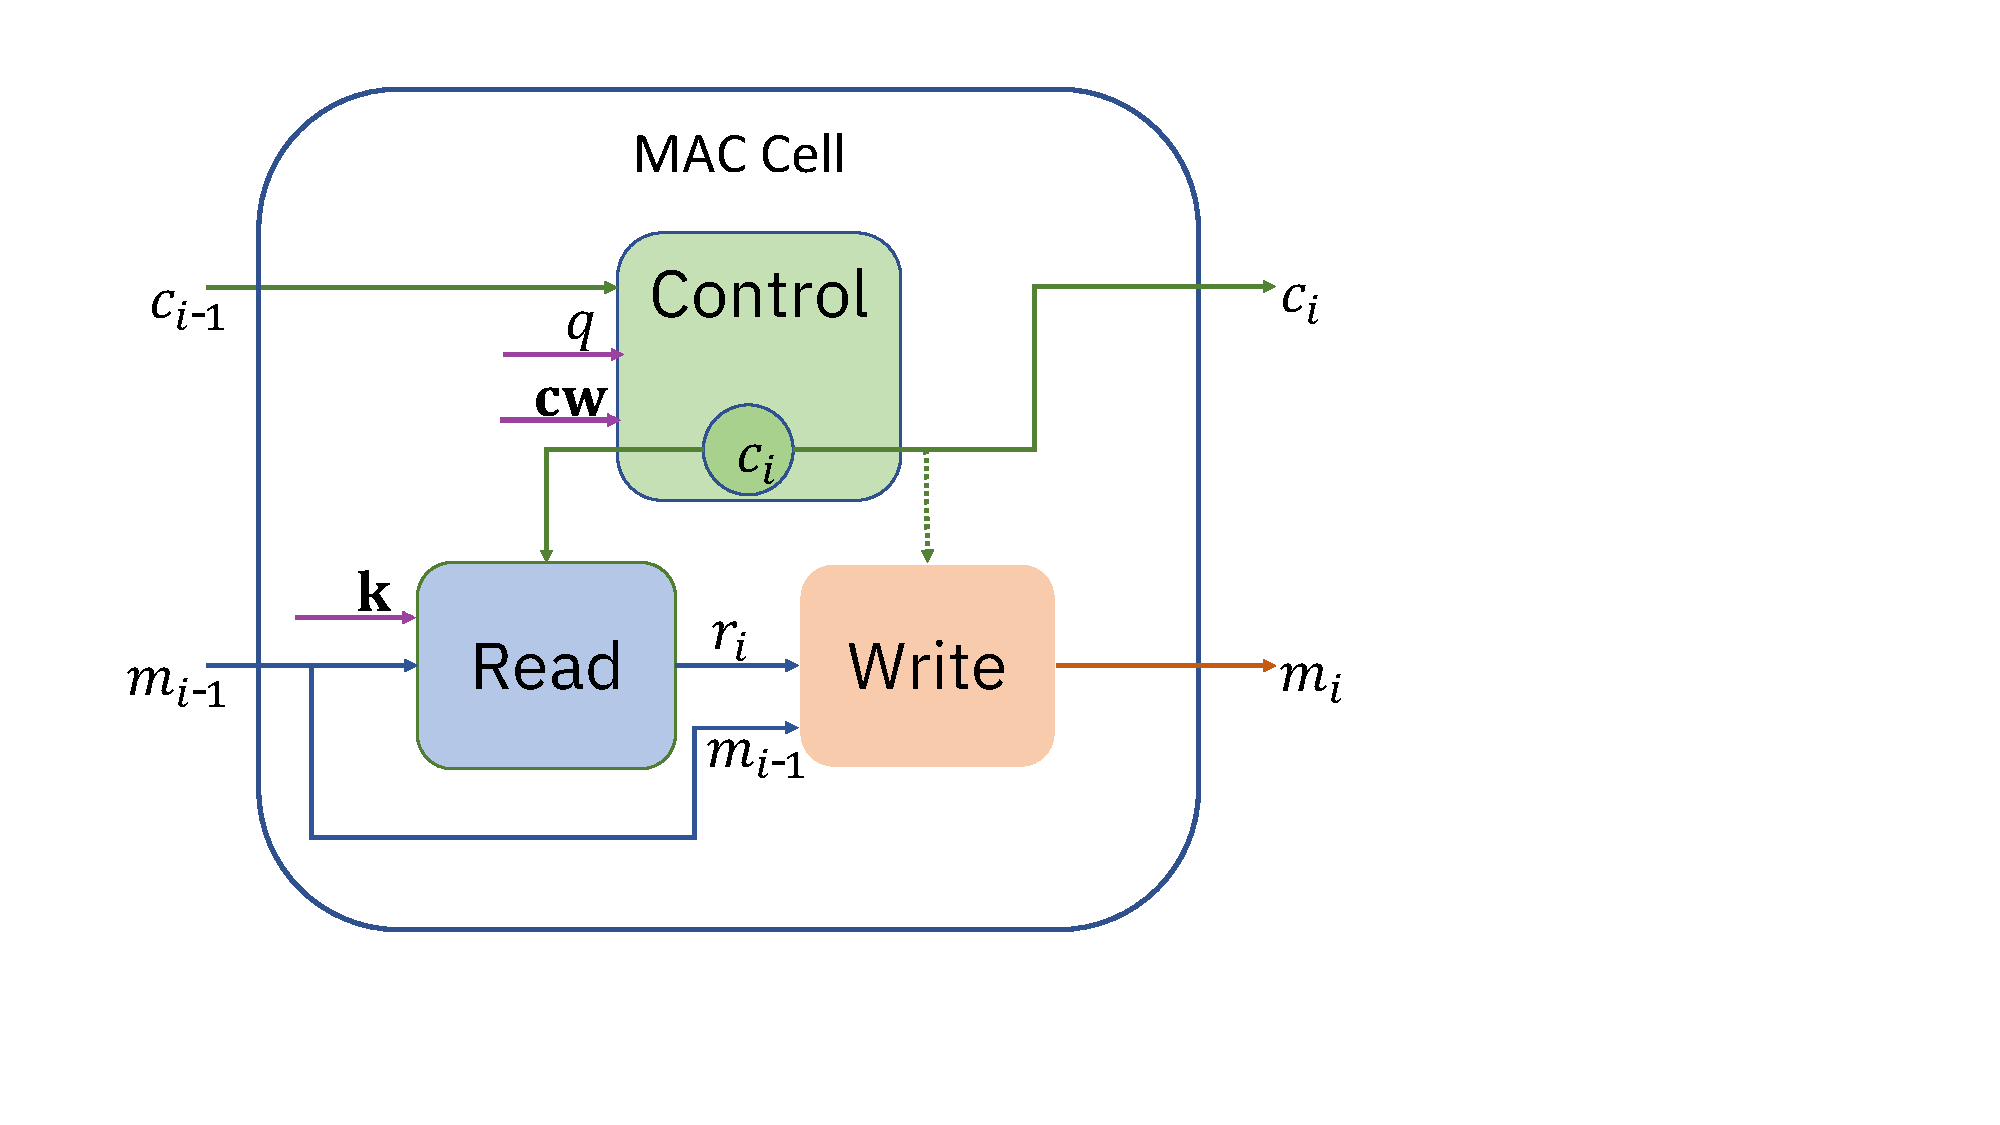
\includegraphics[width=0.60\textwidth]{../img/mac_cell.pdf}
				\label{subfig:pendulum_picture}
		}}
	
		\caption{The MAC cell}
		\label{fig:pendulum}
	\end{figure}
	
The MAC network is a recurrent model that performs sequential reasoning,  where each step involves analyzing a part of the question followed by shifting the attention over the image. The core of the model is the MAC cell, supported with an input unit that processes the question and image pair, and output unit which produces the answer.  The input unit uses an LSTM to process the question in a word-by-word manner producing a sequence of contextual words and a final question representation. Besides, the input unit utilizes a pre-trained ResNet followed by two CNN layers to extract a feature map (referred to as knowledge base) from the image.
}

\headerbox{Simplified Mac Model}{name=data acquisition, column=0, below=double-pendulum}{
	
	Our proposed modification to the MAC network is based on two heuristic simplifications of the
	MAC cell. First, we observe that, taking the MAC cell equations as a whole, consecutive linear
	layers (with no activation in-between) can be combined as one linear layer. Next, we assume that
	dimension-preserving linear layers are invertible so as to avoid information loss. Applying this
	principle to the equations, with a careful reorganization, we can apply a single linear layer to the
	knowledge base prior to all the reasoning steps and work with this projected knowledge base as-is
	throughout the reasoning steps.
	
	
	
	
	
	\begin{table}[H]
		\centering
		\caption{Comparing the number of position-independent parameters between MAC \& S-MAC cells.}
		\begin{tabular}{llll}
			\toprule
			Model        & Read Unit               & Write Unit &  Control Unit         \\
			\midrule
			MAC   &  787,969 &  524,800        &    525,313    \\
			%\midrule
			simplified MAC & 263,168  & 262,656       &    263,168 \\
			\midrule
			Reduction by [\%]  & 67\%  &   50\%       &      50\%  \\
			\bottomrule
		\end{tabular}
		\label{tab:data_properties}
	\end{table}
}

\headerbox{Transfer Learning - Experiments}{name=dataset, column=1}{
	\begin{table}[H]
	\centering
	\scalebox{0.8}{
	\caption{Comparing the number of position-independent parameters between MAC \& S-MAC cells.}
	\begin{tabular}{lllllllll}
		\toprule
		\multirow{2}{*}{Model} & \multicolumn{3}{c}{Training} &  \multicolumn{2}{c}{Fine-tuning} & \multicolumn{2}{c}{Test} & \multirow{2}{*}{Row} \\
		\cmidrule{2-4} \cmidrule{5-6} \cmidrule{7-8} 
		& Dataset                & Time [h:m] & Acc [\%]          & Dataset & Acc [\%]  & Dataset & Acc [\%] & \\
		\midrule
		MAC & CLEVR  & 30:52  & 96.70 & --   & --  & CLEVR    & 96.17         & (a) \\
		\cmidrule{1-8}
		\cmidrule{1-8}
		
		\multirow{13}{*}{S-MAC} & CLEVR  & 28:30  & 95.82 & --   & --  & CLEVR    & 95.29         & (b)  \\
		\cmidrule{2-4} \cmidrule{5-6} \cmidrule{7-8} 
		
		& CoGenT-A  & 28:33   & 96.09 &  --  &  --  & CoGenT-A & 95.91        & (c)  \\
		\cmidrule{2-4} \cmidrule{5-6} \cmidrule{7-8} 
		
		
		& \multirow{2}{*}{CLEVR}  & \multirow{2}{*}{28:30}  & \multirow{2}{*}{95.82} & \multirow{2}{*}{--}   & \multirow{2}{*}{--}  &   CoGenT-A    &  95.47  & (d) \\
		\cmidrule{7-8} 
		&                        &   &              &     &                               & CoGenT-B   &  95.58  & (e)\\		
		
		\cmidrule{2-4} \cmidrule{5-6} \cmidrule{7-8} 
		& \multirow{4}{*}{CoGenT-A}   & \multirow{4}{*}{28:33}   & \multirow{4}{*}{96.09}  &  \multirow{1}{*}{--}  &  \multirow{1}{*}{--}   & CogenT-B & 78.71        & (f)  \\
		\cmidrule{5-6} \cmidrule{7-8} 
		&                             &                                         &    &   \multirow{2}{*}{CoGenT-B}         &       \multirow{2}{*}{96.85}          & CoGenT-A &  91.24        & (g) \\
		\cmidrule{7-8} 
		&                             &                                         &       &         &                & CoGenT-B &    94.55     & (h)  \\
		
		\cmidrule{2-4} \cmidrule{5-6} \cmidrule{7-8} 
		& \multirow{2}{*}{CLEVR}  & \multirow{2}{*}{28:30}  & \multirow{2}{*}{95.82} &   \multirow{2}{*}{CoGenT-B}         &       \multirow{2}{*}{97.67}          & CoGenT-A &  92.11       & (i) \\
		\cmidrule{7-8} 
		&                             &                                         &       &         &                & CoGenT-B &    92.95    & (j)  \\  		
		
		
		\bottomrule
		
	
	\end{tabular}}
	\label{tab:data_properties}
\end{table}
}

\headerbox{MAC failures examples on CLEVR}{name=baseline, column=1, below=dataset}{
	
	
	
	\begin{figure}[H]
	\centering
	\subfloat[]{{
			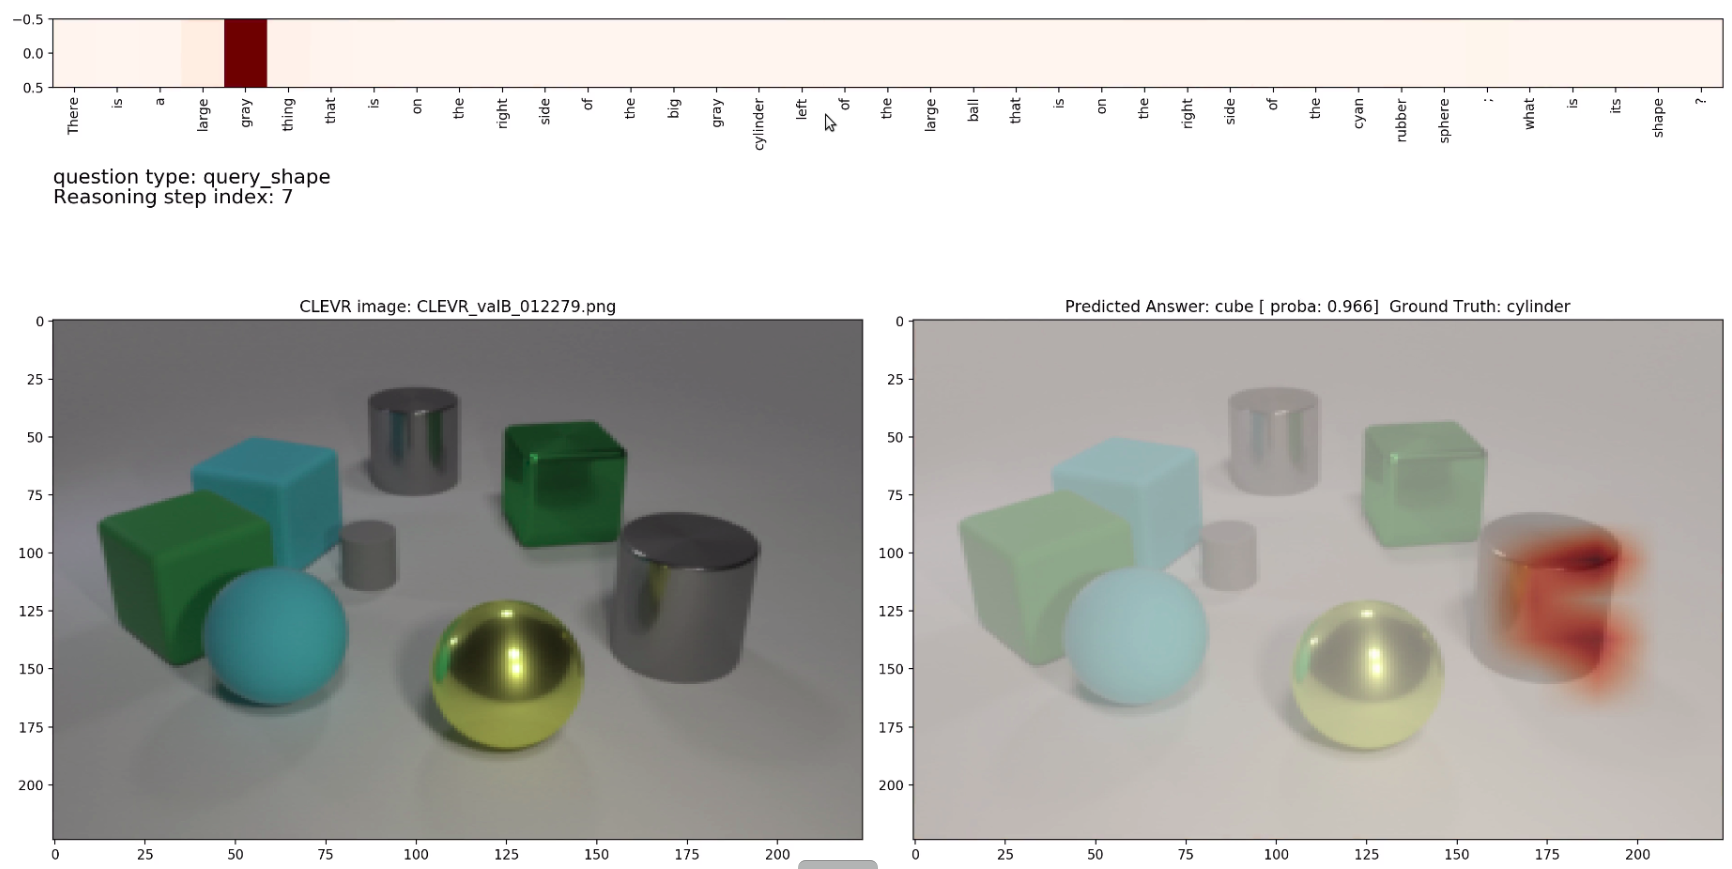
\includegraphics[width=0.9\textwidth]{../img/fail_mac_cogent_b_shape.png}
			\label{subfig:pendulum_picture}
	}}
	
	\caption{The question reads as: \textit{There is a large gray thing that is on the right side of the big gray cylinder left of the large ball that is on the right side if the cyan rubber sphere; what is its shape?}}
	\label{fig:fail_mac_shape}
\end{figure}
	\begin{figure}[H]
	\centering
	\subfloat[]{{
			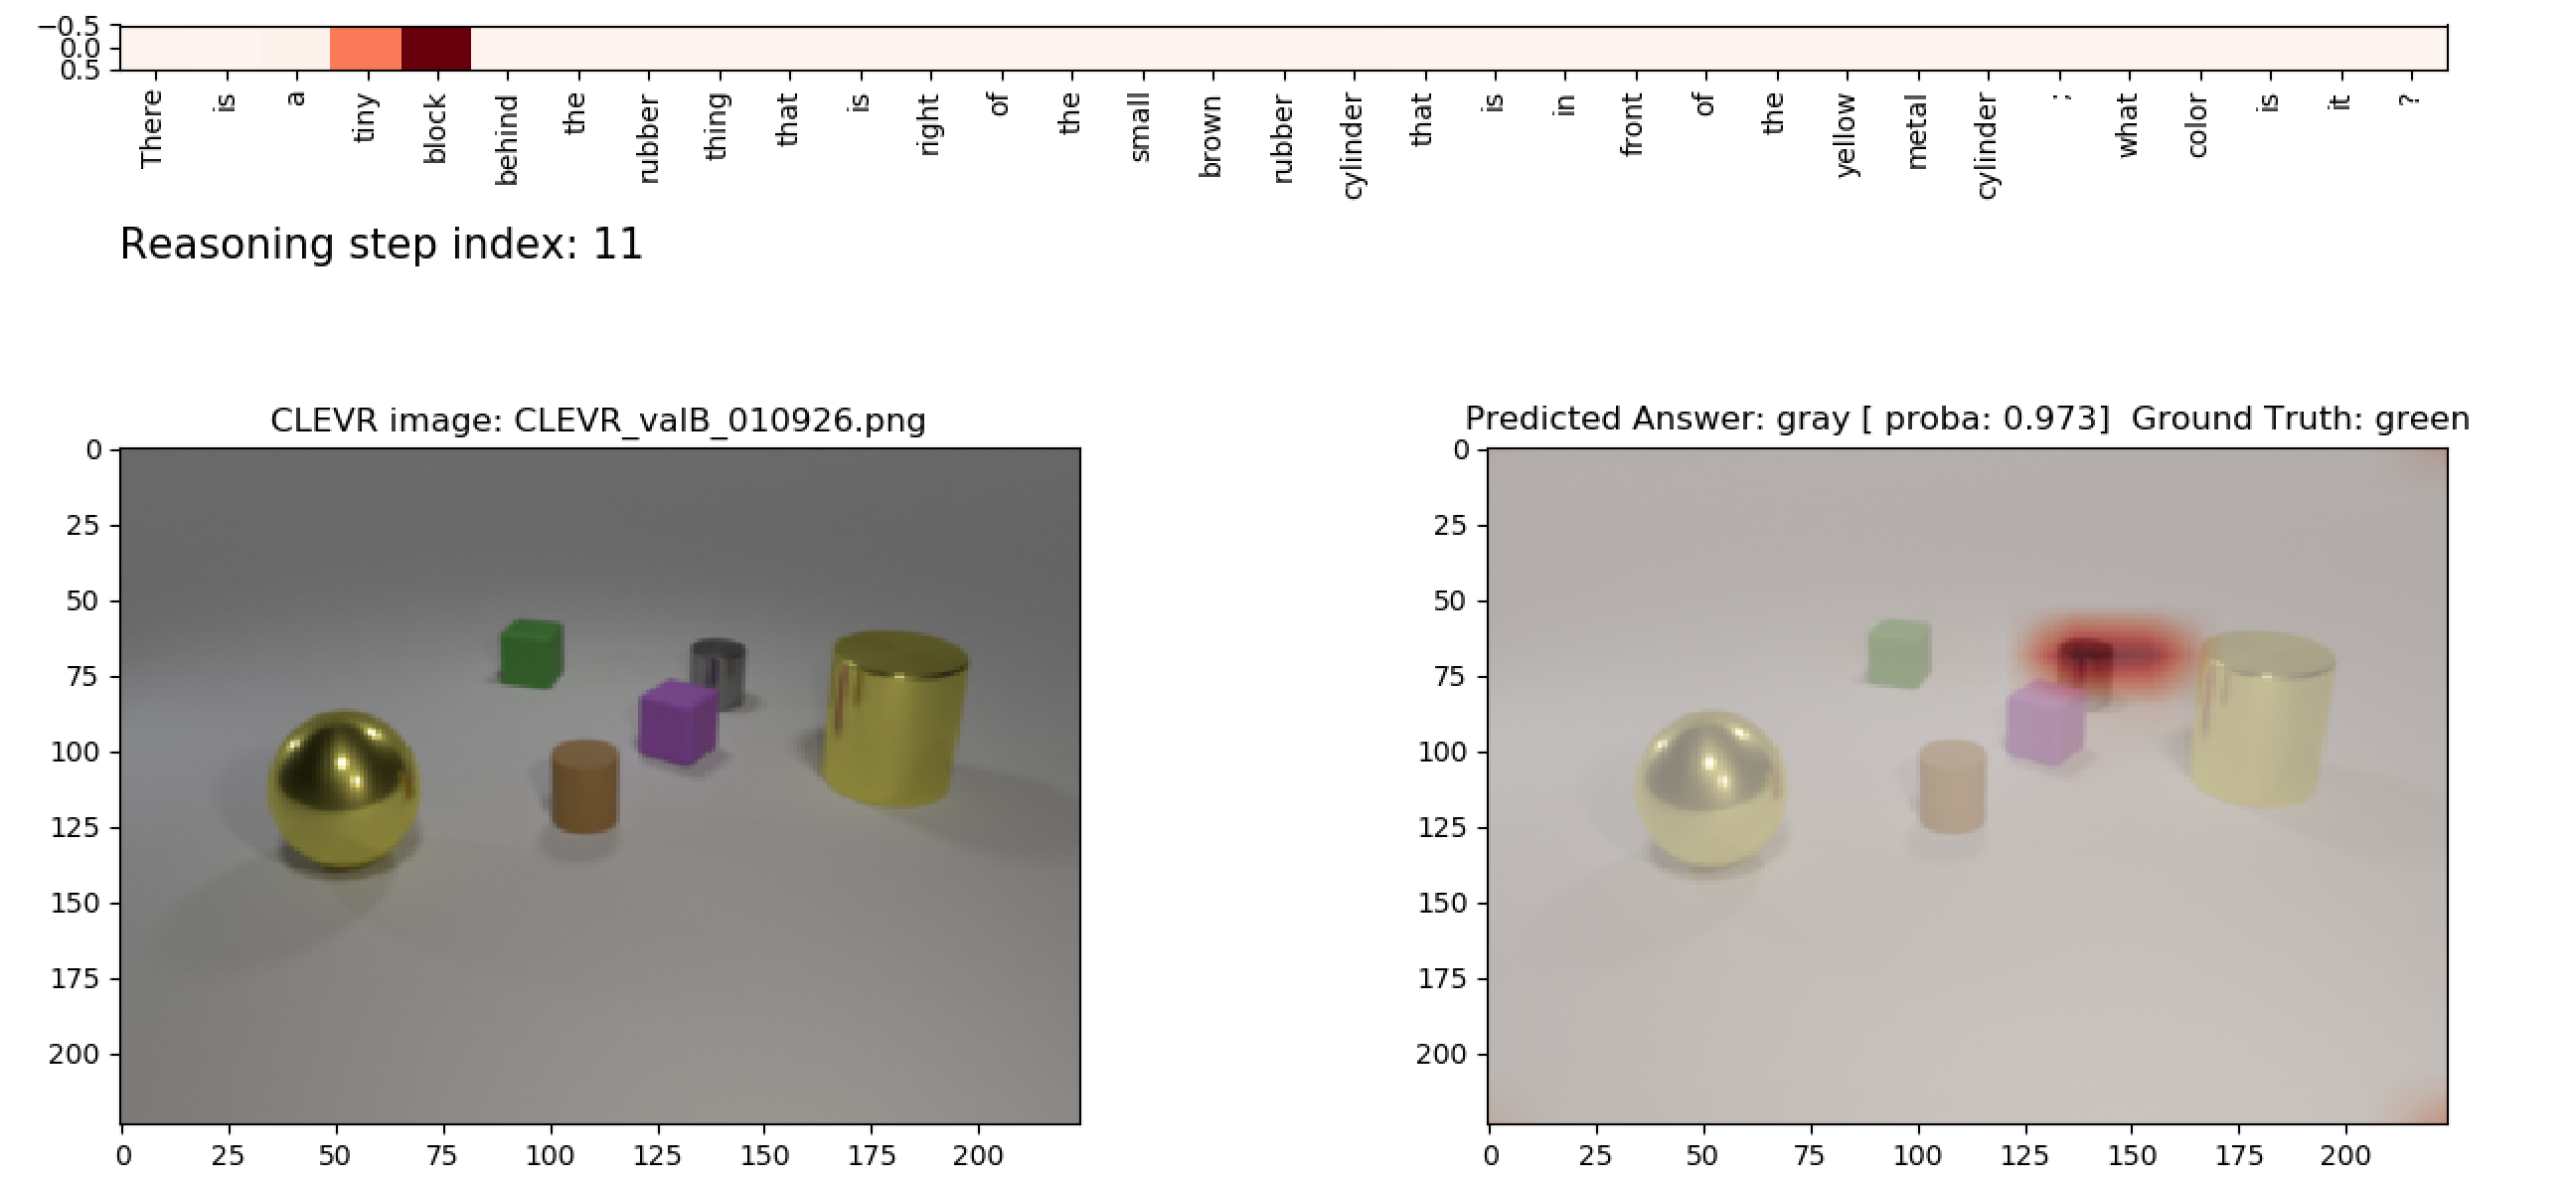
\includegraphics[width=0.9\textwidth]{../img/fail_mac_cogent_b_color.png}
			\label{subfig:pendulum_picture}
	}}
	
	\caption{The question reads as: \textit{There is a tiny block behind the rubber thing that is right if the small brown rubber cylinder that is in front of the yellow metal cylinder; what color is it?}}
    \label{fig:fail_mac_color}
\end{figure}

	


}

\headerbox{References}{name=references, column=1, below=baseline}{


}

\end{poster}

\end{document}